\section{Results} \label{sec:results}

The results of a grounded theory study, as the name of the method itself
suggests, are grounded on the collected data, so the hypotheses emerge from
data. A grounded theory should describe the key relationships between the
categories that compose it, i.e., a set of inter-related hypotheses~\cite{hoda2017becoming}.
We present the categories of our grounded theory
about DevOps adoption as a network of three categories of enablers (\cat{automation},
\cat{sharing} and \cat{transparency}) that are commonly used to develop the core category
\cat{collaboration culture}. Based on our understanding, implementing enablers to develop the \cat{collaboration
culture} typically leads to concepts related to two categories of outcomes:
\cat{agility} and \cat{resilience}. Moreover, there are two categories that can be considered
both as enablers and as outcomes: \cat{continuous measurement} and \cat{quality assurance}.
In this section we describe the relationships between those categories, i.e.,
the hypotheses.

\subsection{How to Adopt DevOps?}

In Section~\ref{sec:introduction} we present the general question of this
research: is there any recommended path to adopt DevOps? Here, we elaborate a response,
based on the analyses conducted as detailed in the previous section. The main
point which should be formulated is the construction of a \cat{collaboration
culture} between the software development and operations teams and
related activities. According to our findings, the other categories,
many of which are also present in other studies that have investigated DevOps,
only make sense if the practices and
concepts related to them either contribute to the level of \cat{collaboration
culture} or lead to the expected consequences of a \cat{collaboration
culture}. This understanding induces several hypothesis, as discussed in
what follows.

\begin{mh}
\textbf{H1:} \textit{There is a group of categories related to DevOps adoption
that only make sense if used to increase the} \cat{collaboration culture} \emph{level. We
call this group of categories of \textbf{enablers}}.
\end{mh}

Based on this first hypothesis, there is no increase in collaboration
level in the situations where only one team is responsible to understand, adapt or
evolve the automation to support (a) deployment activities, (b) infrastructure provisioning and management,
and (c) monitoring activities. In these scenarios, the level of DevOps adoption does not advance.
The same is valid to the other \emph{enabling} categories. That is, in the situations where
\cat{transparency} and \cat{sharing} do not contribute to
the \cat{collaboration culture}, they do not contribute to DevOps adoption as a whole. Next
we present some examples of the underlying raw data that support H1.

\begin{mq}
``\emph{Look, inside the operations sector there was some degree of automation. The guy
had stored in his own machine bash scripts that helped him when setting up a
server or when creating a new database instance. Nevertheless, there was no DevOps
because there was no intrinsic relationship of this automation to the
development process}" (P11, DevOps Supervisor, Brazil)
\end{mq}


\begin{mq}
``\emph{
DevOps involves tooling, but DevOps is not tooling. That is, people often
focus on using tools that are called 'DevOps tools', believing that DevOps is
this. I always insist that DevOps is not use tools, DevOps involves use these
tools properly to improve software development procedures}" (P2, DevOps
Consultant, Brazil)
\end{mq}


\begin{mq}
``\emph{Keeping the culture alive remains a challenge to us, and it is very
important. Here in our company, for example, we have Tech Talks that are
monthly conversations that we have with the teams. The purpose of these Tech
Talks is to share knowledge about technologies and work processes increasing the
transparency of how everything works. We also have a Slack channel called
DevOps as Culture where we discuss things of DevOps culture. The idea is not to
let the culture die, we are always feeding it with something, because that is
the DevOps essence for us.}" (P12, Cloud Engineer, United States)
\end{mq}

\begin{mh}
\textbf{H2:} \textit{There is a group of categories related to DevOps adoption
that does not contribute to increase the} \cat{collaboration culture} \emph{level, but that instead are
pointed out as DevOps adoption related, because they emerge as an expected or
necessary consequence of the adoption. We call this group of categories of
\textbf{outcomes}}.
\end{mh}

In a first moment, the simple fact that a team is more
\cat{agile} in delivering software, or more \cat{resilient} in failure recovery, does not
contribute directly to bring operations teams closer to development teams.
Nevertheless, the respondents of the interviews frequently cited that DevOps
increases the capacity for continuously delivering software (\cat{agile})
and for building \cat{resilient} infrastructures.

{\color{red}examples - esta exemplificado nas categorias, talvez mover para ca
para nao ficar redundante}

\textbf{H3:} \textit{The categories \cat{Continuous Measurement} and \cat{Quality Assurance}
are related both to DevOps enabling capacity and to DevOps outcomes}.
Measurement is cited as a typical responsibility of the operations team.
At the same time that the sharing of this responsibility contributes to reduce the silo,
it is also cited as a necessary consequence after DevOps adoption, because
the context of agility with the continuous delivery of software requires more caution,
which is supplied by concepts related to the \cat{continuous measurement} category.
The same premise is valid to the \cat{quality assurance} category. At first glance,
\cat{quality assurance} appears as one response to the context of agility in operations
provided by DevOps adoption. But, the efforts in quality assurance of software products
increase the confidence between the dev and ops teams increasing the level
of \cat{collaboration culture}.

{\color{red}examples - esta exemplificado nas categorias, talvez mover para ca
para nao ficar redundante}

\subsection{DevOps Enablers}

DevOps enablers are exactly the means commonly used to increase the level of
the \cat{collaboration culture} in a DevOps adoption process.
We have identified five categories of DevOps enablers:
\cat{ Automation}, \cat{Continuous Measurement}, \cat{Quality Assurance},
\cat{Sharing} {\color{red}of what?}, and {\cat{Transparency}.

\textbf{H4:} \textit{There is no precedence between enablers in a DevOps
adoption process}. We have perceived that the adoption process can follow a
path that prioritizes specific enablers, on the condition that the level of
\cat{collaboration culture} increases. In addition, there is no enabler with evidence that
can be more efficient to another in collaboration culture development. For
instance, although 14 respondents cite \cat{automation} as an important
enabler to adopt DevOps, some respondents also ponder that considering
automation with greater importance than other parts can be a risk:

\begin{mq}
``\emph{I think that the expansion of collaboration between teams involved other
things, it was not just automation. There must be an alignment with the
business needs. (...) I think that DevOps made possible a broader understanding
of software production and we were realizing exactly that it is not about
automating everything. What we need is a broader understanding of that task.
Sometimes, we conclude that the task is not completely necessary and then we
solve the problem by changing procedures without the effort necessary to
automate it. So, I see with caution a supposed vision that automate things can
be the way to implement DevOps.}" (P7, Support Analyst, Brazil)
\end{mq}

\begin{mq}
``\emph{Despite of we actually use automation in a reasonable number of scenarios, we have been able to develop our culture significantly without automation and I think that you can reach a good DevOps level with little or even no automation.}" (P8, DevOps Engineer, Brazil)
\end{mq}

That is, although \cat{automation} is a very commonly used enabler, it is possible to
increase the level of \cat{collaboration culture} without focus on automating. And
this premise is valid to the other enablers. {\color{red}Each enabler will be detailed in
the sequence of the paper}.

\subsection{DevOps Outcomes}

DevOps outcomes is that group of categories doesn't produces primarily the
expected effect of a DevOps enabler, typically concepts that are expected as
consequences of an adoption of DevOps. We have identified four categories that
can work as DevOps outcomes: \cat{Agility}, \cat{Continuous Measurement},
\cat{Quality Assurance}, and \cat{Software Resilience}. Note that,
as mentioned before, \cat{Continuous Measurement} and \cat{Quality Assurance}
are both enablers and consequences.

That is, A well succeeded DevOps adoption typically increases the potential of
\cat{agility}, \cat{continuous measurement}, \cat{quality assurance} and
\cat{resilience} of a team {\color{red}resilience of a team or of a software?} .
However, in some situations this potential is not completely used due business
decisions. For example, one respondent cited that, at a first moment, the
company do not allowed the continuous deployment of applications in production:

\begin{mq}
``\emph{We had conditions and security to continuously publish in production,
however, in the beginning the managers were afraid and decided that the
publication would happen weekly.}" (P9, IT Manager, Brazil)
\end{mq}

In this case, DevOps increased the level of agility of the company, but this
potential was not totally achieved. As well as enablers, each outcome
will be detailed in the sequence of the paper.

Based on H1-H4 hypothesis, in Fig. 2 we present a three step model of how to
adopt DevOps according with our proposal.

\begin{itemize}
\item In the first step, a company should  understand and
disseminate that the goal with a DevOps adoption should be
the establishment of a \cat{collaboration culture} between
development and operations teams.

\item In the second step, a company should select and develop
the most suitable enablers according with its context. The enablers
are means commonly used to develop the \cat{collaboration culture}
and its concepts.

\item In the third step, a company should check the outcomes of the
DevOps adoption in order to verify the alignment with
industrial practices and to explore them according to the
need of the company.
\end{itemize}

\begin{figure*}
  \centering
    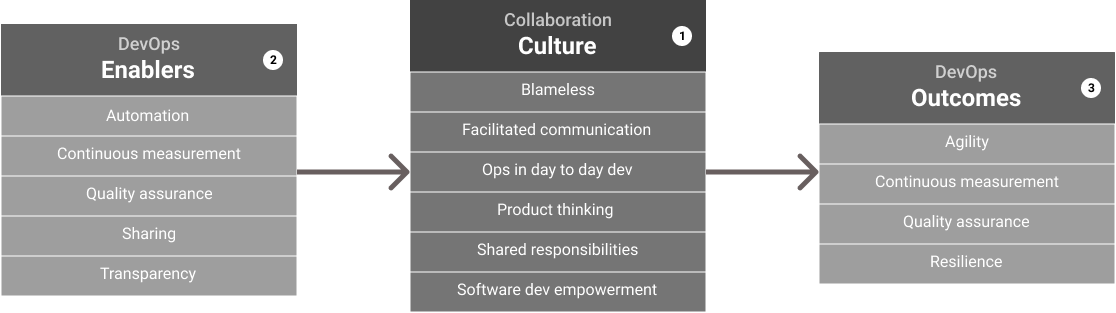
\includegraphics[width=14.26cm,height=4cm,natwidth=1116,natheight=313]{model.png}
    \caption{DevOps Adoption Model}
    \label{fig2}
\end{figure*}
